% A simple template for LaTeX documents
% 
% To produce pdf run:
%   $ pdflatex paper.tex 
%


\documentclass[12pt]{article}

% Begin paragraphs with new line
\usepackage{parskip}  

% Change margin size
\usepackage[margin=1in]{geometry}   

% Graphics Example:  (PDF's make for good plots)
\usepackage{graphicx}               
% \centerline{\includegraphics{figure.pdf}}

% subfigures, side by side
\usepackage{subcaption}

% hyperlinks
\usepackage{hyperref}

% Blocks of code
\usepackage{listings}
\lstset{basicstyle=\ttfamily, title=\lstname}
% Insert code like this. replace `plot.R` with file name.
% \lstinputlisting{plot.R}

% Monospaced fonts
%\usepackage{inconsolata}
% GNU \texttt{make} is a nice tool.

% Supports proof environment
\usepackage{amsthm}

% Allows writing \implies and align*
\usepackage{amsmath}

% Allows mathbb{R}
\usepackage{amsfonts}

% Numbers in scientific notation
% \usepackage{siunitx}

% Use tables generated by pandas
\usepackage{booktabs}

% Allows umlaut and non ascii characters
\usepackage[utf8]{inputenc}

% Insert blank pages
\usepackage{afterpage}
%\afterpage{\null\newpage}

% norm and infinity norm
\newcommand{\norm}[1]{\left\lVert#1\right\rVert}
\newcommand{\inorm}[1]{\left\lVert#1\right\rVert_\infty}

% Statistics essentials
\newcommand{\iid}{\text{ iid }}
\newcommand{\Exp}{\operatorname{E}}
\newcommand{\Var}{\operatorname{Var}}
\newcommand{\Cov}{\operatorname{Cov}}


%%%%%%%%%%%%%%%%%%%%%%%%%%%%%%%%%%%%%%%%%%%%%%%%%%%%%%%%%%%%

\begin{document}

\title{Parallel Computing Through Code Analysis}
\date{\today}
\author{Clark Fitzgerald}
\maketitle

\begin{abstract}

    Conventional systems for parallel programming require users to modify
    existing code to take advantage of a platform's computational
    capabilities, which may include multiprocessing or Graphical Processing
    Units (GPU)s. In this presentation we review the state of the art for
    parallel programming in R and propose code analysis methods to detect
    the potential for parallel execution. The results of the analysis can
    then be used to rewrite and execute semantically equivalent
    instructions efficiently, without requiring the user to modify their
    code. We consider a motivating case study using robust regression to
    analyze the operating characteristics California's highway traffic
    sensor stations on hundreds of gigabytes of traffic sensor data.

\end{abstract}

This is a prospectus for distribution to the committee for PhD
Qualifying Exam in June 2017.

\section{Code, Data, Platform}
%%%%%%%%%%%%%%%%%%%%%%%%%%%%%%%%%%%%%%%%%%%%%%%%%%%%%%%%%%%%

\textbf{Code} is a script to be executed.
\textbf{Data} could be data in memory, single or multiple files, a
memory-mapped file, a database, a parallel file system, etc.
\textbf{Platform} is the computing setup, such as a CPU with 8 cores, a
Spark cluster, or 2 GPUs with a high bandwidth connection. The combination
of (Code, Data, Platform) dictates what strategies should be used for
efficient evaluation. Given this knowledge, our goal is to analyze the
code, potentially reorganizing it for efficient execution on the data and
platform.  This doesn't mean that the system is inventing new algorithms on
the fly.  But it should be capable of tuning existing parameters to the
system at hand. An example of a parameter to be tuned is the chunk size
$n_i$ as described in \ref{section:sequential}.

\section{Motivating Example}
%%%%%%%%%%%%%%%%%%%%%%%%%%%%%%%%%%%%%%%%%%%%%%%%%%%%%%%%%%%%

The California Department of Transportation collects traffic data through
sensors embedded in highways. The sensors measure three quantities: count
of passing vehicles, time during which a vehicle is directly above the
sensor (occupancy), and average velocity \cite{jia2001pems}.  Every thirty
seconds they produce a new data point. $43,680$ sensors in California
measuring 3 parameters multiplied by $(2 \times 60 \times 24)$ measurements
per day results in 377 million new data points per day.  This raw data is
organized into files grouped by (day, district), and is available for
public download.  As an analyst I would like to model velocity as a
function of occupancy for each sensor. This relationship is called the
``fundamental diagram'' within traffic engineering, because it captures the
operating characteristic of this section of road
\cite{daganzo1997fundamentals}.

Robust regression can be used to fit the fundamental diagram, approximating
the integer programming approach to minimize the L1 norm as in
\cite{li2011fundamental}.  From the R language this can be done easily and
efficiently, for example with the \texttt{rlm} (robust linear model)
function in the MASS package \cite{venables2013modern}:

\begin{verbatim}
fit1 = rlm(velocity ~ occupancy, data = station1)
\end{verbatim}

However, the size and organization of the data makes the task much more
difficult.  I've downloaded a subset of the data consisting of measurements
in the San Francisco Bay Area for part of 2016.  It would be easier to
perform the regression if the data were organized in files for each sensor
rather than in files for each day.  One approach then is to reorganize the
data on disk into this file structure. I did this using a simple single
threaded R program, and it took 23 hours to run on 134 GB of data.
Throughput for a conventional hard disk is around 100 MB/s\footnote{RAID,
an array of disks, could make this faster.}, so a lower bound for reading
then writing this reorganized data is approximately $2 * 134000 / 100$
seconds, or 45 minutes. The naive code is 30 times slower than this. So
small inefficiencies add up.

Another drawback is that it requires very specific instructions to
reorganize the data for computations grouped by station. Any parallel
programming will make this even more specific to the data and platform. The
following R code captures the desired semantics:

\begin{verbatim}
by(data, INDICES = station, FUN = piecewise_rlm)
\end{verbatim}

This says group \texttt{data} by \texttt{station}, and apply the
function \texttt{piecewise\_rlm} to each group.

What if we had a system that could inspect the idiomatic R code above that
works on small data sets, and then automatically take steps to scale and to
parallelize the operations? It could also tune them for the specifics of
the system and the data. This is what we're working towards.


\section{Simple Example}
%%%%%%%%%%%%%%%%%%%%%%%%%%%%%%%%%%%%%%%%%%%%%%%%%%%%%%%%%%%%

% Duncan:
% Come up with concrete and realistic examples.  Show how you would do things
% differently for different computational platform Go through this explicitly
% by hand to show the "ideal" transformed code (keep high level) Identify how
% you might identify these programmatically and what are some of the
% challenges

Now we use a simple example to focus on the underlying computational models
to see what can be achieved for large $n$ given various platforms.
Consider computing the mean,

\begin{equation}
    \bar{x} = \frac{1}{n} \sum_{i = 1}^n x_i
\label{eq:mean}
\end{equation}

where the $x_i$'s are
i.i.d. $\sim N(0, 1)$.  In R this code is written:

\begin{verbatim}
xbar = mean(rnorm(n))
\end{verbatim}

To evaluate this R will first build an intermediate vector $x = (x_1,
\dots, x_n)$ and then compute the mean. Eventually that unreferenced
intermediate vector will be garbage collected.
Execution time increases
linearly with $n$. Once $n$ becomes large
enough this vector will no longer fit into available physical memory, so
the operating system will use swap space. On a machine with 8 GB memory
this happens when $O(n) = 10^9$, causing the execution time
to increase by an order of magnitude, roughly from 1 minute to 15
minutes. Once $n$ exceeds memory and swap space R will not be able to allocate a
large enough object, and the computation will fail.

Now we consider alternative ways to execute this code.  Most rely on
splitting the sum into $p$ partial sums with $n_j$ terms each and then rewriting
Equation \ref{eq:mean} as a weighted mean.

\begin{equation}
    \bar{x} = \frac{1}{n} \sum_{j = 1}^p \sum_{i = 1}^{n_j} x_{ij}
    = \sum_{j = 1}^p \frac{n_j}{n} \bar{x}_j
\label{eq:mean_partial}
\end{equation}

It's important to correctly handle the cases when $n$ is not divisible by $p$
and the computation / data cannot be evenly split. For simplicity in the
examples below, suppose that they can be split evenly so $n_i$ is the same
for all $i$.

\subsection{Sequential Execution}
\label{section:sequential}

Equation \ref{eq:mean_partial} can be directly translated into R code as
follows:

\begin{verbatim}

n = 1e5
p = 10
n_i = as.integer(n / p)

meanrnorm = function(n) mean(rnorm(n))

partial_means = sapply(rep(n_i, p), meanrnorm)
xbar = mean(partial_means)
\end{verbatim}

This code does not run in parallel, but it does use the same functional
programming patterns as parallel code. If $M$ is the size of physical memory in
bytes then this code is high performance in the sense
that execution time will continue to be linear while $n < O(M^2)$, just
as it was for small $n < O(M)$. It can also be modified to handle
arbitrarily large $n$. This is because \texttt{sapply} runs
sequentially, so the memory footprint can be bounded since the intermediate
vectors will be of length $n / p$. 

What aspects of the code changed? In the initial code the user
supplied $n$, and it remained to choose $p$ and $n_i$.
The expression \texttt{mean(rnorm(n))} was changed into a function that was
called and reduced using \texttt{mean()}.

\subsection{SNOW cluster}

Clusters created by SNOW, a simple network of workstations consist of independent
worker R processes created by a manager process. The processes communicate
over network sockets, and they may be on one or many physical machines.
This is the type of cluster used by partools \cite{R-partools}.

\begin{verbatim}
cluster = parallel::makeCluster(p)
partial_means = parallel::clusterCall(cluster, meanrnorm, n_i)
xbar = mean(unlist(partial_means))
\end{verbatim}

Given an existing cluster this is very efficient, since we are sending a
few bytes of code over the network and then returning a single number.

\subsection{forking}

On a server capable of forking, for example the department servers which
have as many as 72 cores, one could use this approach. Forking uses a
system fork, which will create several worker processes which can read data from
the manager without copying.

This is inefficient when generating data as we are here, but it's more
efficient if we have already loaded a large data set into the manager
process.

\begin{verbatim}
x = rnorm(n)

starting_indices = as.integer(seq(from = 1, to = n, by = n_i))
ending_indices = starting_indices + (n_i - 1L)

index_mean = function(start, end) mean(x[start:end])

partial_means = parallel::mcmapply(index_mean, starting_indices, ending_indices)

xbar = mean(partial_means)
\end{verbatim}

\subsection{GPU}

The GPU offers the highest level of parallelism, which could consist of
1000's of threads working at once. Following the OpenCL documentation we'll
refer to a GPU as a device, because this can run on other architectures as
well. Here are the simplified steps:

\begin{itemize}
    \item create a kernel which will run in parallel
    \item transfer the data to the device
    \item run the kernel
    \item transfer the results back
\end{itemize}

For this operation the kernel should do the equivalent of the
\texttt{meanrnorm()} function above.  Here's psuedo code for how a kernel
might look in OpenCL, provided the device can fit all of $x$ in memory.
This could be rewritten for larger than device memory by following the
approach in \ref{section:sequential}.

\begin{verbatim}
# include <random.h>

__kernel void meanrnorm(__global float *x
        , __global float *partial_means
        , int n_i
        )
{
    int id = get_global_id(0);

    Random random_state = seed_rand(id);
    int start_index = id * n_i;
    int end_index = start_index + n_i;

    for(int i = start_index; i < end_index; i++)
    {
        random_state = next_rand(random_state);
        x[i] = rnorm(random_state);
    }
    xbar_local = mean(x, start_index, end_index);
    partial_means[id] = xbar_local;
}
\end{verbatim}

This code uses shared memory, since $x$ is a global array.
One can then either write another kernel to reduce
\texttt{partial\_means} on the GPU or return them to the CPU.

\subsection{Threads}

For this problem CPU threads could be utilized in the same way as the GPU.
Indeed, OpenCL was designed to work on multiple platforms including CPU's
and GPU's. The difference is that the memory transfers from host to device
don't take any time, because the host and device are the same.

\subsection{memory mapping}

\subsection{pipelines}

This parallel programming pattern is rather different. A useful analogy is a
factory assembly line, with each worker performing one or more operations
and then passing it to the next worker. The first worker could generate a
subvector of random numbers and pass it along. Ignoring the setup and
looping over chunks the important parts of the code are:

\begin{verbatim}
# Worker 1

x_chunk = rnorm(n_i)
serialize(x_chunk, worker2)
\end{verbatim}

The second worker receives the random numbers and computes the mean.

\begin{verbatim}
# Worker 2

x_chunk = unserialize(worker1)
partial_means[i] = mean(x_chunk)
i = i + 1
\end{verbatim}

This approach is sensible if the load can be balanced across the workers.
Each function should take approximately the same amount of time, and the
overhead required to pass between workers must be much smaller than the
time spent doing work. These assumptions do not all hold in this case,
since if $n = 1000$ then \texttt{xchunk = rnorm(n)} takes 125 $\mu s$,
\texttt{mean(x\_chunk)} takes 6 $\mu s$, and serialization takes at least
15 $\mu s$. On a practical level this can all be implemented over network
sockets or through MPI.


Many of the performance characteristics of the different platforms can be
understood in terms of the overhead to set them up, then the latency and
bandwidth as data is transferred.

\section{Issues}
%%%%%%%%%%%%%%%%%%%%%%%%%%%%%%%%%%%%%%%%%%%%%%%%%%%%%%%%%%%%

How to interface between existing systems? Where to pick up

A layered view of the architecture:

\begin{verbatim}
User layer: foreach, future, partools, ddR
R Foundational layer: SNOW, multicore, (parallel)
System Foundational layers: *NIX fork(), processes, network sockets
\end{verbatim}

\section{Small Data and Overhead}
%%%%%%%%%%%%%%%%%%%%%%%%%%%%%%%%%%%%%%%%%%%%%%%%%%%%%%%%%%%%

For principled approaches to parallel chunked computations we
first have to understand their performance characteristics.

If the data is ``small enough'' then performance will be acceptable no
matter regardless of how well the platform is utilized and how efficient
the code is. Conversely, if the data is ``large enough'' then
\emph{everything} matters, since small inefficiencies will be magnified
when they occur millions of times.

\begin{figure}
\centering
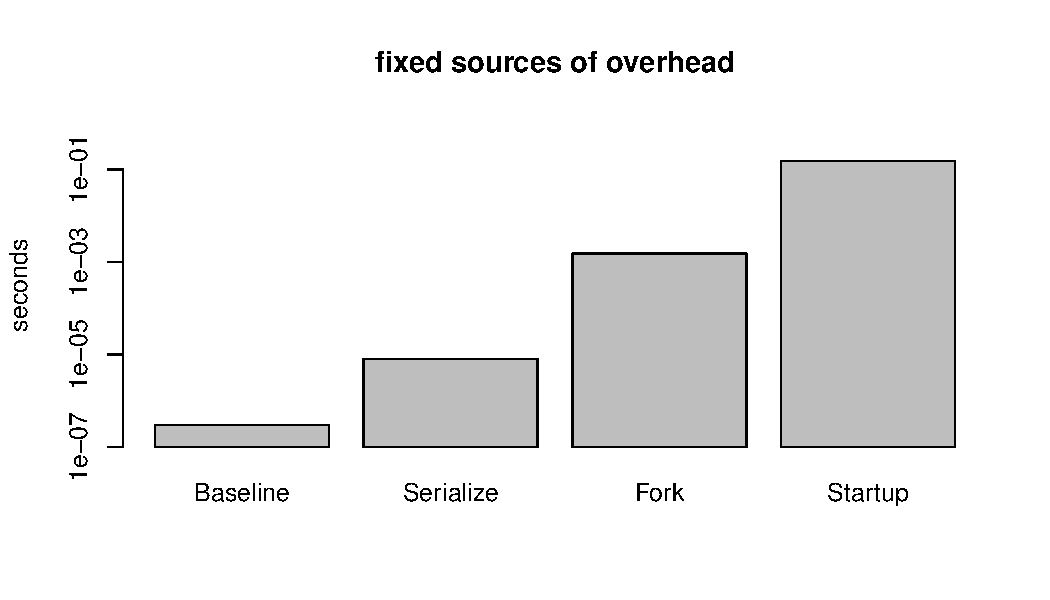
\includegraphics[width=.8\linewidth]{compute_times/overhead}
\caption{Simple function calls take less than a microsecond. Launching a
    new R interpreter takes hundreds of milliseconds, which is relatively expensive.}
\label{fig:overhead}
\end{figure}

Figure \ref{fig:overhead} compares the relative fixed sources of overhead to
consider with parallel programming. The evaluation of the following simple
function captures the basic overhead associated with an interpreted
language like R.
\begin{verbatim}
twox = function(x) 2*x
\end{verbatim}
Every call to this function will incur a fixed overhead that is a couple
hundred nanoseconds. 




\section{Code analysis}
%%%%%%%%%%%%%%%%%%%%%%%%%%%%%%%%%%%%%%%%%%%%%%%%%%%%%%%%%%%%

Code analysis is critical to this approach, and we build on the approaches
developed for compiling R \cite{lang2014enhancing}.

\subsection{Apply functions}

The obvious way to make code parallel is to search for the use of
apply functions and transform them into the parallel versions. For example, 
\texttt{lapply()} can be replaced with \texttt{mclapply()} from the
parallel package to use fork based parallelism.

\subsection{Reduce functions}

\texttt{mean()} as used in \texttt{mean(rnorm(n))} reduces a vector to a
single number. It can 

\subsection{Vectorization}

Goes hand in hand with loop fusion.

\subsection{Dependency Analysis}


\bibliographystyle{plain}
\bibliography{../citations,../Rpackages} 

\end{document}
